\documentclass[12pt,a4paper,]{book}
\def\ifdoblecara{} %% set to true
\def\ifprincipal{} %% set to true
\let\ifprincipal\undefined %% set to false
\def\ifcitapandoc{} %% set to true
\let\ifcitapandoc\undefined %% set to false
\usepackage{lmodern}
% sin fontmathfamily
\usepackage{amssymb,amsmath}
\usepackage{ifxetex,ifluatex}
%\usepackage{fixltx2e} % provides \textsubscript %PLLC
\ifnum 0\ifxetex 1\fi\ifluatex 1\fi=0 % if pdftex
  \usepackage[T1]{fontenc}
  \usepackage[utf8]{inputenc}
\else % if luatex or xelatex
  \ifxetex
    \usepackage{mathspec}
  \else
    \usepackage{fontspec}
  \fi
  \defaultfontfeatures{Ligatures=TeX,Scale=MatchLowercase}
\fi
% use upquote if available, for straight quotes in verbatim environments
\IfFileExists{upquote.sty}{\usepackage{upquote}}{}
% use microtype if available
\IfFileExists{microtype.sty}{%
\usepackage{microtype}
\UseMicrotypeSet[protrusion]{basicmath} % disable protrusion for tt fonts
}{}
\usepackage[margin = 2.5cm]{geometry}
\usepackage{hyperref}
\hypersetup{unicode=true,
            pdfauthor={Nombre Completo Autor},
              pdfborder={0 0 0},
              breaklinks=true}
\urlstyle{same}  % don't use monospace font for urls
%
\usepackage[usenames,dvipsnames]{xcolor}  %new PLLC
\IfFileExists{parskip.sty}{%
\usepackage{parskip}
}{% else
\setlength{\parindent}{0pt}
\setlength{\parskip}{6pt plus 2pt minus 1pt}
}
\setlength{\emergencystretch}{3em}  % prevent overfull lines
\providecommand{\tightlist}{%
  \setlength{\itemsep}{0pt}\setlength{\parskip}{0pt}}
\setcounter{secnumdepth}{5}
% Redefines (sub)paragraphs to behave more like sections
\ifx\paragraph\undefined\else
\let\oldparagraph\paragraph
\renewcommand{\paragraph}[1]{\oldparagraph{#1}\mbox{}}
\fi
\ifx\subparagraph\undefined\else
\let\oldsubparagraph\subparagraph
\renewcommand{\subparagraph}[1]{\oldsubparagraph{#1}\mbox{}}
\fi

%%% Use protect on footnotes to avoid problems with footnotes in titles
\let\rmarkdownfootnote\footnote%
\def\footnote{\protect\rmarkdownfootnote}


  \title{}
    \author{Nombre Completo Autor}
      \date{18/11/2021}


%%%%%%% inicio: latex_preambulo.tex PLLC


%% UTILIZA CODIFICACIÓN UTF-8
%% MODIFICARLO CONVENIENTEMENTE PARA USARLO CON OTRAS CODIFICACIONES


%\usepackage[spanish,es-nodecimaldot,es-noshorthands]{babel}
\usepackage[spanish,es-nodecimaldot,es-noshorthands,es-tabla]{babel}
% Ver: es-tabla (en: https://osl.ugr.es/CTAN/macros/latex/contrib/babel-contrib/spanish/spanish.pdf)
% es-tabla (en: https://tex.stackexchange.com/questions/80443/change-the-word-table-in-table-captions)
\usepackage[spanish, plain, datebegin,sortcompress,nocomment,
noabstract]{flexbib}
 
\usepackage{float}
\usepackage{placeins}
\usepackage{fancyhdr}
% Solucion: ! LaTeX Error: Command \counterwithout already defined.
% https://tex.stackexchange.com/questions/425600/latex-error-command-counterwithout-already-defined
\let\counterwithout\relax
\let\counterwithin\relax
\usepackage{chngcntr}
%\usepackage{microtype}  %antes en template PLLC
\usepackage[utf8]{inputenc}
\usepackage[T1]{fontenc} % Usa codificación 8-bit que tiene 256 glyphs

%\usepackage[dvipsnames]{xcolor}
%\usepackage[usenames,dvipsnames]{xcolor}  %new
\usepackage{pdfpages}
%\usepackage{natbib}




% Para portada: latex_paginatitulo_mod_ST02.tex (inicio)
\usepackage{tikz}
\usepackage{epigraph}
\renewcommand\epigraphflush{flushright}
\renewcommand\epigraphsize{\normalsize}
\setlength\epigraphwidth{0.7\textwidth}

\definecolor{titlepagecolor}{cmyk}{1,.60,0,.40}

%\DeclareFixedFont{\titlefont}{T1}{ppl}{b}{it}{0.5in}

% \makeatletter
% \def\printauthor{%
%     {\large \@author}}
% \makeatother
% \author{%
%     Author 1 name \\
%     Department name \\
%     \texttt{email1@example.com}\vspace{20pt} \\
%     Author 2 name \\
%     Department name \\
%     \texttt{email2@example.com}
%     }

% The following code is borrowed from: https://tex.stackexchange.com/a/86310/10898

\newcommand\titlepagedecoration{%
\begin{tikzpicture}[remember picture,overlay,shorten >= -10pt]

\coordinate (aux1) at ([yshift=-15pt]current page.north east);
\coordinate (aux2) at ([yshift=-410pt]current page.north east);
\coordinate (aux3) at ([xshift=-4.5cm]current page.north east);
\coordinate (aux4) at ([yshift=-150pt]current page.north east);

\begin{scope}[titlepagecolor!40,line width=12pt,rounded corners=12pt]
\draw
  (aux1) -- coordinate (a)
  ++(225:5) --
  ++(-45:5.1) coordinate (b);
\draw[shorten <= -10pt]
  (aux3) --
  (a) --
  (aux1);
\draw[opacity=0.6,titlepagecolor,shorten <= -10pt]
  (b) --
  ++(225:2.2) --
  ++(-45:2.2);
\end{scope}
\draw[titlepagecolor,line width=8pt,rounded corners=8pt,shorten <= -10pt]
  (aux4) --
  ++(225:0.8) --
  ++(-45:0.8);
\begin{scope}[titlepagecolor!70,line width=6pt,rounded corners=8pt]
\draw[shorten <= -10pt]
  (aux2) --
  ++(225:3) coordinate[pos=0.45] (c) --
  ++(-45:3.1);
\draw
  (aux2) --
  (c) --
  ++(135:2.5) --
  ++(45:2.5) --
  ++(-45:2.5) coordinate[pos=0.3] (d);   
\draw 
  (d) -- +(45:1);
\end{scope}
\end{tikzpicture}%
}

% Para portada: latex_paginatitulo_mod_ST02.tex (fin)

% Para portada: latex_paginatitulo_mod_OV01.tex (inicio)
\usepackage{cpimod}
% Para portada: latex_paginatitulo_mod_OV01.tex (fin)

% Para portada: latex_paginatitulo_mod_OV03.tex (inicio)
\usepackage{KTHEEtitlepage}
% Para portada: latex_paginatitulo_mod_OV03.tex (fin)

\renewcommand{\contentsname}{Índice}
\renewcommand{\listfigurename}{Índice de figuras}
\renewcommand{\listtablename}{Índice de tablas}
\newcommand{\bcols}{}
\newcommand{\ecols}{}
\newcommand{\bcol}[1]{\begin{minipage}{#1\linewidth}}
\newcommand{\ecol}{\end{minipage}}
\newcommand{\balertblock}[1]{\begin{alertblock}{#1}}
\newcommand{\ealertblock}{\end{alertblock}}
\newcommand{\bitemize}{\begin{itemize}}
\newcommand{\eitemize}{\end{itemize}}
\newcommand{\benumerate}{\begin{enumerate}}
\newcommand{\eenumerate}{\end{enumerate}}
\newcommand{\saltopagina}{\newpage}
\newcommand{\bcenter}{\begin{center}}
\newcommand{\ecenter}{\end{center}}
\newcommand{\beproof}{\begin{proof}} %new
\newcommand{\eeproof}{\end{proof}} %new
%De: https://texblog.org/2007/11/07/headerfooter-in-latex-with-fancyhdr/
% \fancyhead
% E: Even page
% O: Odd page
% L: Left field
% C: Center field
% R: Right field
% H: Header
% F: Footer
%\fancyhead[CO,CE]{Resultados}

%OPCION 1
% \fancyhead[LE,RO]{\slshape \rightmark}
% \fancyhead[LO,RE]{\slshape \leftmark}
% \fancyfoot[C]{\thepage}
% \renewcommand{\headrulewidth}{0.4pt}
% \renewcommand{\footrulewidth}{0pt}

%OPCION 2
% \fancyhead[LE,RO]{\slshape \rightmark}
% \fancyfoot[LO,RE]{\slshape \leftmark}
% \fancyfoot[LE,RO]{\thepage}
% \renewcommand{\headrulewidth}{0.4pt}
% \renewcommand{\footrulewidth}{0.4pt}
%%%%%%%%%%
\usepackage{calc,amsfonts}
% Elimina la cabecera de páginas impares vacías al finalizar los capítulos
\usepackage{emptypage}
\makeatletter

%\definecolor{ocre}{RGB}{25,25,243} % Define el color azul (naranja) usado para resaltar algunas salidas
\definecolor{ocre}{RGB}{0,0,0} % Define el color a negro (aparece en los teoremas

%\usepackage{calc} 


%era if(csl-refs) con dolares
% metodobib: true


\usepackage{lipsum}

%\usepackage{tikz} % Requerido para dibujar formas personalizadas

%\usepackage{amsmath,amsthm,amssymb,amsfonts}
\usepackage{amsthm}


% Boxed/framed environments
\newtheoremstyle{ocrenumbox}% % Theorem style name
{0pt}% Space above
{0pt}% Space below
{\normalfont}% % Body font
{}% Indent amount
{\small\bf\sffamily\color{ocre}}% % Theorem head font
{\;}% Punctuation after theorem head
{0.25em}% Space after theorem head
{\small\sffamily\color{ocre}\thmname{#1}\nobreakspace\thmnumber{\@ifnotempty{#1}{}\@upn{#2}}% Theorem text (e.g. Theorem 2.1)
\thmnote{\nobreakspace\the\thm@notefont\sffamily\bfseries\color{black}---\nobreakspace#3.}} % Optional theorem note
\renewcommand{\qedsymbol}{$\blacksquare$}% Optional qed square

\newtheoremstyle{blacknumex}% Theorem style name
{5pt}% Space above
{5pt}% Space below
{\normalfont}% Body font
{} % Indent amount
{\small\bf\sffamily}% Theorem head font
{\;}% Punctuation after theorem head
{0.25em}% Space after theorem head
{\small\sffamily{\tiny\ensuremath{\blacksquare}}\nobreakspace\thmname{#1}\nobreakspace\thmnumber{\@ifnotempty{#1}{}\@upn{#2}}% Theorem text (e.g. Theorem 2.1)
\thmnote{\nobreakspace\the\thm@notefont\sffamily\bfseries---\nobreakspace#3.}}% Optional theorem note

\newtheoremstyle{blacknumbox} % Theorem style name
{0pt}% Space above
{0pt}% Space below
{\normalfont}% Body font
{}% Indent amount
{\small\bf\sffamily}% Theorem head font
{\;}% Punctuation after theorem head
{0.25em}% Space after theorem head
{\small\sffamily\thmname{#1}\nobreakspace\thmnumber{\@ifnotempty{#1}{}\@upn{#2}}% Theorem text (e.g. Theorem 2.1)
\thmnote{\nobreakspace\the\thm@notefont\sffamily\bfseries---\nobreakspace#3.}}% Optional theorem note

% Non-boxed/non-framed environments
\newtheoremstyle{ocrenum}% % Theorem style name
{5pt}% Space above
{5pt}% Space below
{\normalfont}% % Body font
{}% Indent amount
{\small\bf\sffamily\color{ocre}}% % Theorem head font
{\;}% Punctuation after theorem head
{0.25em}% Space after theorem head
{\small\sffamily\color{ocre}\thmname{#1}\nobreakspace\thmnumber{\@ifnotempty{#1}{}\@upn{#2}}% Theorem text (e.g. Theorem 2.1)
\thmnote{\nobreakspace\the\thm@notefont\sffamily\bfseries\color{black}---\nobreakspace#3.}} % Optional theorem note
\renewcommand{\qedsymbol}{$\blacksquare$}% Optional qed square
\makeatother



% Define el estilo texto theorem para cada tipo definido anteriormente
\newcounter{dummy} 
\numberwithin{dummy}{section}
\theoremstyle{ocrenumbox}
\newtheorem{theoremeT}[dummy]{Teorema}  % (Pedro: Theorem)
\newtheorem{problem}{Problema}[chapter]  % (Pedro: Problem)
\newtheorem{exerciseT}{Ejercicio}[chapter] % (Pedro: Exercise)
\theoremstyle{blacknumex}
\newtheorem{exampleT}{Ejemplo}[chapter] % (Pedro: Example)
\theoremstyle{blacknumbox}
\newtheorem{vocabulary}{Vocabulario}[chapter]  % (Pedro: Vocabulary)
\newtheorem{definitionT}{Definición}[section]  % (Pedro: Definition)
\newtheorem{corollaryT}[dummy]{Corolario}  % (Pedro: Corollary)
\theoremstyle{ocrenum}
\newtheorem{proposition}[dummy]{Proposición} % (Pedro: Proposition)


\usepackage[framemethod=default]{mdframed}



\newcommand{\intoo}[2]{\mathopen{]}#1\,;#2\mathclose{[}}
\newcommand{\ud}{\mathop{\mathrm{{}d}}\mathopen{}}
\newcommand{\intff}[2]{\mathopen{[}#1\,;#2\mathclose{]}}
\newtheorem{notation}{Notation}[chapter]


\mdfdefinestyle{exampledefault}{%
rightline=true,innerleftmargin=10,innerrightmargin=10,
frametitlerule=true,frametitlerulecolor=green,
frametitlebackgroundcolor=yellow,
frametitlerulewidth=2pt}


% Theorem box
\newmdenv[skipabove=7pt,
skipbelow=7pt,
backgroundcolor=black!5,
linecolor=ocre,
innerleftmargin=5pt,
innerrightmargin=5pt,
innertopmargin=10pt,%5pt
leftmargin=0cm,
rightmargin=0cm,
innerbottommargin=5pt]{tBox}

% Exercise box	  
\newmdenv[skipabove=7pt,
skipbelow=7pt,
rightline=false,
leftline=true,
topline=false,
bottomline=false,
backgroundcolor=ocre!10,
linecolor=ocre,
innerleftmargin=5pt,
innerrightmargin=5pt,
innertopmargin=10pt,%5pt
innerbottommargin=5pt,
leftmargin=0cm,
rightmargin=0cm,
linewidth=4pt]{eBox}	

% Definition box
\newmdenv[skipabove=7pt,
skipbelow=7pt,
rightline=false,
leftline=true,
topline=false,
bottomline=false,
linecolor=ocre,
innerleftmargin=5pt,
innerrightmargin=5pt,
innertopmargin=10pt,%0pt
leftmargin=0cm,
rightmargin=0cm,
linewidth=4pt,
innerbottommargin=0pt]{dBox}	

% Corollary box
\newmdenv[skipabove=7pt,
skipbelow=7pt,
rightline=false,
leftline=true,
topline=false,
bottomline=false,
linecolor=gray,
backgroundcolor=black!5,
innerleftmargin=5pt,
innerrightmargin=5pt,
innertopmargin=10pt,%5pt
leftmargin=0cm,
rightmargin=0cm,
linewidth=4pt,
innerbottommargin=5pt]{cBox}

% Crea un entorno para cada tipo de theorem y le asigna un estilo 
% con ayuda de las cajas coloreadas anteriores
\newenvironment{theorem}{\begin{tBox}\begin{theoremeT}}{\end{theoremeT}\end{tBox}}
\newenvironment{exercise}{\begin{eBox}\begin{exerciseT}}{\hfill{\color{ocre}\tiny\ensuremath{\blacksquare}}\end{exerciseT}\end{eBox}}				  
\newenvironment{definition}{\begin{dBox}\begin{definitionT}}{\end{definitionT}\end{dBox}}	
\newenvironment{example}{\begin{exampleT}}{\hfill{\tiny\ensuremath{\blacksquare}}\end{exampleT}}		
\newenvironment{corollary}{\begin{cBox}\begin{corollaryT}}{\end{corollaryT}\end{cBox}}	

%	ENVIRONMENT remark
\newenvironment{remark}{\par\vspace{10pt}\small 
% Espacio blanco vertical sobre la nota y tamaño de fuente menor
\begin{list}{}{
\leftmargin=35pt % Indentación sobre la izquierda
\rightmargin=25pt}\item\ignorespaces % Indentación sobre la derecha
\makebox[-2.5pt]{\begin{tikzpicture}[overlay]
\node[draw=ocre!60,line width=1pt,circle,fill=ocre!25,font=\sffamily\bfseries,inner sep=2pt,outer sep=0pt] at (-15pt,0pt){\textcolor{ocre}{N}}; \end{tikzpicture}} % R naranja en un círculo (Pedro)
\advance\baselineskip -1pt}{\end{list}\vskip5pt} 
% Espaciado de línea más estrecho y espacio en blanco después del comentario


\newenvironment{solutionExe}{\par\vspace{10pt}\small 
\begin{list}{}{
\leftmargin=35pt 
\rightmargin=25pt}\item\ignorespaces 
\makebox[-2.5pt]{\begin{tikzpicture}[overlay]
\node[draw=ocre!60,line width=1pt,circle,fill=ocre!25,font=\sffamily\bfseries,inner sep=2pt,outer sep=0pt] at (-15pt,0pt){\textcolor{ocre}{S}}; \end{tikzpicture}} 
\advance\baselineskip -1pt}{\end{list}\vskip5pt} 

\newenvironment{solutionExa}{\par\vspace{10pt}\small 
\begin{list}{}{
\leftmargin=35pt 
\rightmargin=25pt}\item\ignorespaces 
\makebox[-2.5pt]{\begin{tikzpicture}[overlay]
\node[draw=ocre!60,line width=1pt,circle,fill=ocre!55,font=\sffamily\bfseries,inner sep=2pt,outer sep=0pt] at (-15pt,0pt){\textcolor{ocre}{S}}; \end{tikzpicture}} 
\advance\baselineskip -1pt}{\end{list}\vskip5pt} 

\usepackage{tcolorbox}

\usetikzlibrary{trees}

\theoremstyle{ocrenum}
\newtheorem{solutionT}[dummy]{Solución}  % (Pedro: Corollary)
\newenvironment{solution}{\begin{cBox}\begin{solutionT}}{\end{solutionT}\end{cBox}}	


\newcommand{\tcolorboxsolucion}[2]{%
\begin{tcolorbox}[colback=green!5!white,colframe=green!75!black,title=#1] 
 #2
 %\tcblower  % pone una línea discontinua
\end{tcolorbox}
}% final definición comando

\newtcbox{\mybox}[1][green]{on line,
arc=0pt,outer arc=0pt,colback=#1!10!white,colframe=#1!50!black, boxsep=0pt,left=1pt,right=1pt,top=2pt,bottom=2pt, boxrule=0pt,bottomrule=1pt,toprule=1pt}



\mdfdefinestyle{exampledefault}{%
rightline=true,innerleftmargin=10,innerrightmargin=10,
frametitlerule=true,frametitlerulecolor=green,
frametitlebackgroundcolor=yellow,
frametitlerulewidth=2pt}





\newcommand{\betheorem}{\begin{theorem}}
\newcommand{\eetheorem}{\end{theorem}}
\newcommand{\bedefinition}{\begin{definition}}
\newcommand{\eedefinition}{\end{definition}}

\newcommand{\beremark}{\begin{remark}}
\newcommand{\eeremark}{\end{remark}}
\newcommand{\beexercise}{\begin{exercise}}
\newcommand{\eeexercise}{\end{exercise}}
\newcommand{\beexample}{\begin{example}}
\newcommand{\eeexample}{\end{example}}
\newcommand{\becorollary}{\begin{corollary}}
\newcommand{\eecorollary}{\end{corollary}}


\newcommand{\besolutionExe}{\begin{solutionExe}}
\newcommand{\eesolutionExe}{\end{solutionExe}}
\newcommand{\besolutionExa}{\begin{solutionExa}}
\newcommand{\eesolutionExa}{\end{solutionExa}}


%%%%%%%%


% Caja Salida Markdown
\newmdenv[skipabove=7pt,
skipbelow=7pt,
rightline=false,
leftline=true,
topline=false,
bottomline=false,
backgroundcolor=GreenYellow!10,
linecolor=GreenYellow!80,
innerleftmargin=5pt,
innerrightmargin=5pt,
innertopmargin=10pt,%5pt
innerbottommargin=5pt,
leftmargin=0cm,
rightmargin=0cm,
linewidth=4pt]{mBox}	

%% RMarkdown
\newenvironment{markdownsal}{\begin{mBox}}{\end{mBox}}	

\newcommand{\bmarkdownsal}{\begin{markdownsal}}
\newcommand{\emarkdownsal}{\end{markdownsal}}


\usepackage{array}
\usepackage{multirow}
\usepackage{wrapfig}
\usepackage{colortbl}
\usepackage{pdflscape}
\usepackage{tabu}
\usepackage{threeparttable}
\usepackage{subfig} %new
%\usepackage{booktabs,dcolumn,rotating,thumbpdf,longtable}
\usepackage{dcolumn,rotating}  %new
\usepackage[graphicx]{realboxes} %new de: https://stackoverflow.com/questions/51633434/prevent-pagebreak-in-kableextra-landscape-table

%define el interlineado vertical
%\renewcommand{\baselinestretch}{1.5}

%define etiqueta para las Tablas o Cuadros
%\renewcommand\spanishtablename{Tabla}

%%\bibliographystyle{plain} %new no necesario


%%%%%%%%%%%% PARA USO CON biblatex
% \DefineBibliographyStrings{english}{%
%   backrefpage = {ver pag.\adddot},%
%   backrefpages = {ver pags.\adddot}%
% }

% \DefineBibliographyStrings{spanish}{%
%   backrefpage = {ver pag.\adddot},%
%   backrefpages = {ver pags.\adddot}%
% }
% 
% \DeclareFieldFormat{pagerefformat}{\mkbibparens{{\color{red}\mkbibemph{#1}}}}
% \renewbibmacro*{pageref}{%
%   \iflistundef{pageref}
%     {}
%     {\printtext[pagerefformat]{%
%        \ifnumgreater{\value{pageref}}{1}
%          {\bibstring{backrefpages}\ppspace}
%          {\bibstring{backrefpage}\ppspace}%
%        \printlist[pageref][-\value{listtotal}]{pageref}}}}
% 
%%% de kableExtra
\usepackage{booktabs}
\usepackage{longtable}
%\usepackage{array}
%\usepackage{multirow}
%\usepackage{wrapfig}
%\usepackage{float}
%\usepackage{colortbl}
%\usepackage{pdflscape}
%\usepackage{tabu}
%\usepackage{threeparttable}
\usepackage{threeparttablex}
\usepackage[normalem]{ulem}
\usepackage{makecell}
%\usepackage{xcolor}

%%%%%%% fin: latex_preambulo.tex PLLC


\begin{document}

\bibliographystyle{flexbib}



\raggedbottom

\ifdefined\ifprincipal
\else
\setlength{\parindent}{1em}
\pagestyle{fancy}
\setcounter{tocdepth}{4}
\tableofcontents

\fi

\ifdefined\ifdoblecara
\fancyhead{}{}
\fancyhead[LE,RO]{\scriptsize\rightmark}
\fancyfoot[LO,RE]{\scriptsize\slshape \leftmark}
\fancyfoot[C]{}
\fancyfoot[LE,RO]{\footnotesize\thepage}
\else
\fancyhead{}{}
\fancyhead[RO]{\scriptsize\rightmark}
\fancyfoot[LO]{\scriptsize\slshape \leftmark}
\fancyfoot[C]{}
\fancyfoot[RO]{\footnotesize\thepage}
\fi

\renewcommand{\headrulewidth}{0.4pt}
\renewcommand{\footrulewidth}{0.4pt}

\hypertarget{preliminares}{%
\chapter{Preliminares}\label{preliminares}}

En este capítulo se introducirán los elementos principales que sientan
las bases de las técnicas empleadas en el estudio junto con las
herramientas computacionales utilizadas, aspectos esenciales para el
adecuado seguimiento y comprensión del resto del documento.

\hypertarget{datos-georreferenciados}{%
\section{Datos georreferenciados}\label{datos-georreferenciados}}

Todos los datos empleados en este trabajo son georreferenciados, lo que
significa que están asociados a ubicaciones geográficas específicas. Por
ello, resulta esencial introducir los tipos de datos más utilizados para
trabajar con esta información, sus características y las herramientas
disponibles para manipularlos. En esta sección se tratarán los datos
vectoriales y los datos ráster, al ser los tipos fundamentales en este
contexto, con características bien diferenciadas entre ellos.

\hypertarget{datos-vectoriales}{%
\subsection{Datos vectoriales}\label{datos-vectoriales}}

El modelo de datos vectoriales se basa en puntos ubicados dentro de un
sistema de referencia de coordenadas (CRS, por sus siglas en inglés).
Estos puntos pueden representar características independientes o pueden
estar conectados para formar geometrías más complejas como líneas y
polígonos. Para esta sección se han usado como referencia
\citep{lovelace_geocomputation_2019} y \citep{introGISGimond}.

\hypertarget{simple-features}{%
\subsubsection*{\texorpdfstring{\emph{Simple
Features}}{Simple Features}}\label{simple-features}}

Las \emph{Simple Features} son un estándar abierto ampliamente utilizado
para la representación de datos vectoriales, desarrollado y respaldado
por el \emph{Open Geospatial Consortium} (OGC), una organización sin
ánimo de lucro dedicada a la creación de estándares abiertos e
interoperables a nivel global dentro del marco de los sistemas
geográficos de información (GIS, por sus siglas en ingés) y de la
\emph{World Wide Web} \citep{OCGweb}.

El paquete \emph{sf} proporciona en \emph{R} clases para datos
vectoriales geográficos y una interfaz de línea de comandos consistente
para importantes bibliotecas de bajo nivel para geoprocesamiento
(\emph{GDAL}, \emph{PROJ}, \emph{GEOS}, \emph{S2},\ldots)
\citep{sfpackage}.

Los objetos \emph{sf} son fáciles de manipular, ya que son
\emph{dataframes} o \emph{tibbles} con dos características
fundamentales. En primer lugar, contienen metadatos geográficos
adicionales: tipo de geometría, dimensión, \emph{Bounding Box} (límites
o extensión geográfica) e información sobre el Sistema de referencia de
coordenadas. Además, presentan una columna de geometrías, que contiene
los atributos geográficos de cada observación. Algunas ventajas del uso
de este modelo de datos en \(R\) son que en la mayoría de operaciones
los objetos \emph{sf} se pueden tratar como \emph{dataframes}, los
nombres de las funciones son consistentes (todos empiezan por
\texttt{st\_}), las funciones se pueden combinar con el operador tubería
y además funcionan bien con el ecosistema de paquetes \emph{tidyverse}.

El paquete \emph{sf} de \(R\) admite 18 tipos de geometrías para las
\emph{simple features}, de las cuales las más utilizadas se muestran en
la Figura \ref{fig:sf-classes}.

\begin{figure}[H]
\centering
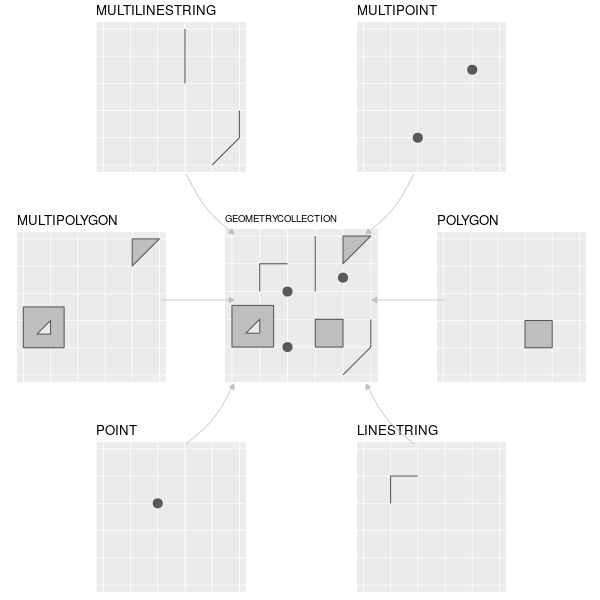
\includegraphics[width = 0.7\textwidth]{graficos/sf-classes.png}
\caption[Principales tipos de \textit{simple features} soportados por el paquete de \textit{R sf}]{Principales tipos de \textit{simple features} soportados por el paquete de \textit{R sf}. \it Fuente: \citet{lovelace_geocomputation_2019}.}
\label{fig:sf-classes}
\end{figure}

\hypertarget{datos-ruxe1ster}{%
\subsection{Datos ráster}\label{datos-ruxe1ster}}

El modelo de datos ráster representa el espacio con una cuadrícula de
celdas (o píxeles), a cada una de las cuales se le asocia un valor o
varios, tratándose así de rásteres de una o varias capas,
respectivamente. Lo más común es trabajar con cuadrículas regulares, es
decir, formadas por celdas rectangulares de igual tamaño. Sin embargo,
existen otros modelos de ráster más complejos en los que se usan
cuadrículas irregulares (rotadas, truncadas, rectilíneas o curvilíneas)
\citep{lovelace_geocomputation_2019}.

Los datos en formato ráster constan de una cabecera y una matriz cuyos
elementos representan celdas equiespaciadas. En la cabecera del ráster
se definen el sistema de referencia de coordenadas, la extensión (o
límites espaciales del área cubierta por el ráster), la resolución y el
origen. El origen son las coordenadas de uno de los píxeles del ráster,
que sirve de referencia para los demás, siendo generalmente utilizado el
de la esquina inferior izquierda \footnote{Sin embargo, el paquete
  \emph{TERRA}, usado en este trabajo, usa por defecto el de la esquina
  superior izquierda \citep{terrapackage}}. La resolución se calcula
como:

\[ resolution = \left(\frac{x_{max}-x_{min}}{ncol},\frac{y_{max}-y_{min}}{nrow}\right) \]

La representación en forma de matriz evita tener que almacenar
explícitamente las coordenadas de cada una de las cuatro esquinas de
cada píxel, debiendo almacenar solamente las coordenadas de un punto (el
origen). Esto hace que el procesamiento de datos ráster sea mucho más
eficiente que el de datos vectoriales.

Se usará el paquete \emph{TERRA} para tratar los datos en formato
ráster, que permite tratar el modelo de rásteres regulares con una o
varias capas a través de la clase de objetos \texttt{SpatRaster}.

\hypertarget{sistemas-de-referencia-de-coordenadas}{%
\subsection{Sistemas de Referencia de
Coordenadas}\label{sistemas-de-referencia-de-coordenadas}}

Intrínseco a cualquier modelo de datos espaciales está el concepto de
Sistema de Referencia de Coordenadas (CRS), que establece cómo la
geometría de los datos se relaciona con la superficie terrestre. Es
decir, es el nexo de unión entre el modelo de datos y la realidad, por
lo que juega un papel fundamental. Los CRS pueden ser de dos tipos:
geográficos o proyectados. En esta sección se usan como referencia el
Capítulo 9 de \citep{introGISGimond} y el Capítulo 2 de
\citep{lovelace_geocomputation_2019}.

\hypertarget{sistemas-de-coordenadas-geogruxe1ficas}{%
\subsubsection*{Sistemas de Coordenadas
Geográficas}\label{sistemas-de-coordenadas-geogruxe1ficas}}

Los sistemas de coordenadas geográficas (GCS) identifican cada punto de
la superficie terrestre utilizando la longitud y la latitud. La longitud
es la distancia angular al Meridiano de Greenwich medida en la dirección
Este-Oeste. La latitud es la distancia angular al Ecuador medida en la
dirección Sur-Norte.

Cualquier sistema de coordenadas geográficas se compone de tres
elementos: el elipsoide, el geoide y el \emph{datum}. El primero, el
elipsoide o esfera, es utilizado para representar de forma simplificada
la superficie terrestre; sobre él se supone que se encuentran los datos
y es el que permitirá realizar mediciones. El segundo, el geoide, es el
modelo matemático que representa la verdadera forma de la Tierra, que no
es suave sino que presenta ondulaciones debidas a las fluctuaciones del
campo gravitatorio a lo largo de la superficie terrestre, las cuales
también cambian a una amplia escala temporal. Por último, el
\emph{datum}, indica cómo se alinean el elipsoide y el geoide, es decir,
cómo el modelo matemático se ajusta a la realidad. Este puede ser local
o geocéntrico, en función de si el elipsoide se ajusta al geoide en un
punto concreto de la superficie terrestre o de si es el centro del
elipsoide el que se alinea con el centro de la Tierra. Ejemplos de
\emph{datum} geocéntricos usados en este trabajo son:

\begin{itemize}
\tightlist
\item
  \emph{European Terrestrial Reference System 1989} (ETRS89), usado
  ampliamente en la Europa Occidental.
\item
  \emph{World Geodetic System 1984} (WGS84), usado a nivel global
  \citep{lovelace_geocomputation_2019}.
\end{itemize}

\hypertarget{sistemas-de-coordenadas-proyectadas}{%
\subsubsection*{Sistemas de Coordenadas
Proyectadas}\label{sistemas-de-coordenadas-proyectadas}}

Un Sistema de Coordenadas Proyectadas (PCS) es un sistema de referencia
que permite identificar localizaciones terrestres y realizar mediciones
en una superficie plana, es decir, en un mapa. Estos sistemas de
coordenadas se basan en las coordenadas cartesianas, por lo que tienen
un origen, un eje X y un eje Y y usan una unidad lineal de medida (en
este trabajo se usará el metro). Pasar de una superficie elíptica (GCR)
a una superficie plana (PCS) requiere de transformaciones matemáticas
apropiadas y siempre induce deformaciones en los datos.

Al proyectar la superficie terrestre en una superficie plana siempre se
modifican algunas propiedades de los objetos, como el área, la
dirección, la distancia o la forma. Un PCS solo puede conservar alguna
de estas propiedades pero no todas, por lo que es habitual clasificar
los PCS en función de la propiedad que mantienen: las proyecciones de
igual área preservan el área, las azimutales preservan la dirección, las
equidistantes preservan la distancia y las conformales preservan la
forma local. En función de cómo se realice la proyección, estas también
se pueden clasificar en planas, cilíndricas o cónicas.

Un caso particular y ampliamente usado de PCS cilíndrico son los
\emph{Universe Transverse Mercator} (UTM), en los que se proyecta el
elipsoide sobre un cilindro tangente a este por las líneas de longitud
(los meridianos). De esta forma, se divide el globo en 60 zonas de
\(6^\circ\) de longitud, para cada una de las cuales existe un PCS UTM
correspondiente que está asociado al meridiano central. Se trata de
proyecciones conformales, por lo que preservan ángulos y formas en
pequeñas regiones, pero distorsionan distancias y áreas.

A lo largo de este trabajo se utilizará el sistema de coordenadas
proyectadas UTM30N, ya que es el que traen muchos de los archivos ráster
manipulados, y es conveniente evitar cambiar de CRS los datos ráster
siempre que sea posible, ya que esta operación provoca una pérdida de
información.

\hypertarget{anuxe1lisis-exploratorio-de-datos}{%
\section{Análisis Exploratorio de
Datos}\label{anuxe1lisis-exploratorio-de-datos}}

El Análisis Exploratorio de Datos (EDA) es una parte fundamental de todo
proyecto de \emph{Machine Learning}, y en general de cualquier proyecto
en el que se deba trabajar con datos de cualquier procedencia para
extraer de ellos conclusiones. Antes del procesamiento de los datos es
siempre necesario explorar, entender y evaluar la calidad de estos, pues
como indica la expresión inglesa \emph{garbage in, garbage out}, si
trabajamos con datos pobres, no podemos esperar obtener de ellos buenos
resultados \citep{wickham2016r}.

El EDA hace referencia al conjunto de técnicas estadísticas (tanto
numéricas como gráficas) con las que se pretende explorar, describir y
resumir la naturaleza de los datos, comprender las relaciones existentes
entre las distintas variables presentes, identificar posibles errores o
revelar posibles valores atípicos, todo esto con el objetivo de
maximizar nuestra compresión sobre el conjunto de datos.

\hypertarget{depuraciuxf3n-de-los-datos}{%
\subsection{Depuración de los datos}\label{depuraciuxf3n-de-los-datos}}

La depuración de los datos o \emph{data cleaning} es el proceso de
detectar y corregir o eliminar datos incorrectos, corruptos, con formato
inadecuado, duplicados o incompletos dentro de un conjunto de datos.
Puede considerarse una fase dentro del EDA (como se sugiere en
\citep{wickham2016r}) o una fase previa a este.

Puede entenderse que el \emph{data cleaning} es el proceso de pasar de
\emph{raw data} o datos en bruto a datos técnicamente correctos y
finalmente a datos consistentes.

\begin{figure}[H]
\centering
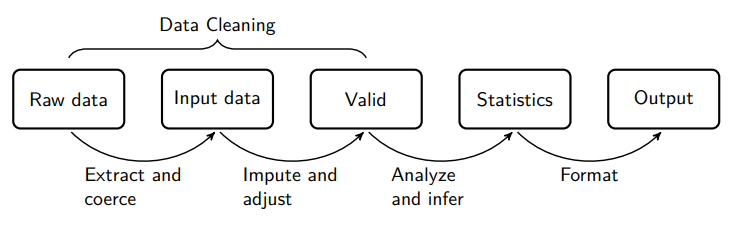
\includegraphics[width = 0.85\textwidth]{graficos/statistical_value_chain.png}
\caption[Etapas en el procesamiento de los datos dentro de un proyecto estadístico]{Etapas en el procesamiento de los datos dentro de un proyecto estadístico. \it Fuente: \citet{van2018statistical}.}
\label{fig:stat_val}
\end{figure}

Entendemos que un conjunto de datos es técnicamente correcto cuando cada
valor pertenece a una variable y está almacenado en el tipo que le
corresponde en base al conocimiento del dominio del problema. Para ello
se debe reajustar el tipo de cada variable al que le corresponda en base
al conocimiento que se tenga sobre esta, codificando los valores en las
clases adecuadas si fuese necesario.

Decimos que un conjunto de datos es consistente cuando es técnicamente
correcto y, además, adecuado para el análisis estadístico. Se trata, por
tanto, de datos que han eliminado, corregido o imputado los valores
faltantes, los valores especiales, los valores atípicos y los errores
\citep{de2013introduction}.

\hypertarget{anuxe1lisis-de-componentes-principales}{%
\subsection{Análisis de Componentes
Principales}\label{anuxe1lisis-de-componentes-principales}}

El Análisis de Componentes Principales (PCA) es una técnica de reducción
de la dimensionalidad ampliamente usada en el análisis de datos
multivariante. Al emplear técnicas de reducción de dimensionalidad como
PCA, se persiguen diversos objetivos: eliminar correlaciones
redundantes, reducir el ruido presente en los datos y facilitar el uso
de algoritmos cuya eficiencia computacional está fuertemente
influenciada por la dimensionalidad de los datos. A continuación, se
definen los conceptos fundamentales del Análisis de Componentes
Principales siguiendo el enfoque expuesto en \citep{PCAShaoDeng}.

\begin{definition}
Dadas $\underline x_1, ..., \underline x_n \in \mathbb{R}^k$ realizaciones de un vector aleatorio $\underline X$ en $\mathbb{R}^k$, se dice que los vectores $\underline c_1, \underline c_2,...,\underline c_p \in \mathbb{R}^k$ son las $k$ componentes principales (muestrales) del vector aleatorio $\underline X$ si forman una base ortonormal del espacio $V \subset \mathbb{R}^k$ de dimensión $p$ que minimiza la media del cuadrado de la distancia euclídea entre los $\underline x_i$ y su proyección $\pi_{V}(\underline x_i)$ sobre $V$.
\end{definition}

De la propia definición se desprende que las componentes principales no
son únicas.

\begin{proposition}
Las $p$ primeras componentes principales se corresponden con los autovectores unitarios asociados a los $p$ mayores autovalores $\lambda_j$ de la matriz de covarianzas muestrales. 
\end{proposition}

\begin{definition}
Se define la fracción de varianza explicada por las $p$ primeras componentes principales, con $p \le k$, como $\frac{\sum_{j=1}^p \lambda_j}{\sum_{j=1}^k \lambda_j}$.
\end{definition}

El número de componentes principales necesarias para explicar un
porcentaje elevado de la varianza de los datos puede servir para
caracterizar la complejidad del problema, indicando la verdadera
dimensión en la que se encuentran los datos.

\hypertarget{modelos}{%
\section{Modelos}\label{modelos}}

El problema que se aborda en este trabajo se engloba dentro de lo que se
conoce como aprendizaje supervisado, ya que para cada observación del
conjunto de entrenamiento se conoce el valor de la variable objetivo (en
este caso si ha habido incendio o no). Más concretamente, se trata de un
problema de clasificación binaria, ya que el objetivo es asignar cada
observación a una de las dos clases posibles (incendio o no incendio).
Existen numerosas técnicas de clasificación binaria supervisada, y en
este trabajo se explorarán algunas de las de uso más común en problemas
similares. Las principales fuentes consultadas para esta sección han
sido \citep{hastie2009elements} y el capítulo 6 de
\citep{MLmodelSuthaharan}. Para entender la intuición detrás de los
modelos puede ser útil el blog \citep{eight2late}.

\hypertarget{regresiuxf3n-loguxedstica-con-penalizaciuxf3n}{%
\subsection{Regresión Logística con
penalización}\label{regresiuxf3n-loguxedstica-con-penalizaciuxf3n}}

La Regresión Logística es un caso particular de Modelo Lineal
Generalizado basado en las siguientes hipótesis:

\begin{itemize}
\tightlist
\item
  \textbf{Hipótesis distribucional}. Dadas las variables explicativas,
  \(\underline X_i\) con \(i = 1,2,...,n\), se verifica que las
  variables \(Y|_{\underline X= \underline x_i}\) son independientes y
  su distribución pertenece a la familia Bernouilli, es decir,
\end{itemize}

\[Y|_{\underline X= \underline x_i} \sim Be(\pi( \underline x_i))\]

\begin{itemize}
\tightlist
\item
  \textbf{Hipótesis estructural}. La esperanzara
  \(E(Y|_{\underline X = \underline x_i}) = \pi_i\), donde
  \(\pi_i = \pi( \underline x_i)\), está relacionada con un predictor
  lineal (\(\eta_i = \beta^t z_i\)) a través de la función \emph{logit}
  con parámetro \(\underline z_i = \left(1,\underline x_i\right)\). Es
  decir, dado que
  \[\eta_i = \underline \beta^t \underline z_i= \ln\left(\frac{\pi_i}{1-\pi_i}\right)\]
  O equivalentemente,
  \[\pi_i = \frac{\exp(\underline \beta^t \underline z_i)}{1 + \exp(\underline \beta^t \underline z_i)}\]
\end{itemize}

Bajo estas hipótesis, la función de log-verosimilitud dada una muestra
\(\{ (\underline x_i,y_i) \}_{i=1,...,n}\) es:

\[ l(\underline \beta) = 
\sum_{i=1}^n \left[ 
y_i\ln \left( \frac{\pi_i}{1-\pi_i} \right) + 
\ln \left( 1 - \pi_i\right) \right]\]

En la Regresión Logística clásica se estima el vector de parámetros
\(\underline \beta\) maximizando la función de log-verosimilud, o lo que
es equivalente, minimizando su opuesta. Por tanto, el problema de
optimización a resolver será
\[\min_{\underline \beta} -l(\underline \beta)\]

Sin embargo, con el objetivo de evitar el sobreajuste y construir
modelos con mayor capacidad de generalización, existen variaciones de la
Regresión Logística que incluyen un término de penalización en la
función objetivo. Las dos variantes de uso más extendido son las
regresiones \emph{ridge} y \emph{lasso}.

Sea \(\underline \beta = \left( \beta_0, \underline \beta_1 \right)\),
donde \(\underline \beta_1\) contiene los coeficientes de las
covariables. En la regresión \emph{ridge} el término de penalización es
de la forma \(\| \underline \beta_1 \|^2_2\), mientras que en la
regresión \emph{lasso} es de la forma \(\| \underline \beta_1 \|_1\).
Por tanto, el problema de optimización asociado será

\[\min_{\underline \beta} -l(\underline \beta)  + \lambda \sum \beta_i^2 \]

en el caso de la regresión logística \emph{ridge} y

\[\min_{\underline \beta} -l(\underline \beta)  + \lambda \sum |\beta_i|\]

en el caso de la Regresión Logística \emph{lasso}, donde en ambos casos
\(\lambda\) es un parámetro de regularización o de penalización.

En este trabajo se usará el paquete \emph{glmnet} \citep{glmnetpackage},
que implementa una combinación de ambos métodos (llamada \emph{elastic
net}), en la que se añade un parámetro de mezcla
\(\alpha \in \left[0,1\right]\) que combina ambos enfoques. El problema
de optimización resultante en este caso será:

\[\min_{\underline \beta} -l(\underline \beta)  + \lambda \left[(1-\alpha)\sum \beta_i^2 + \alpha \sum |\beta_i| \right]\]

\hypertarget{muxe1quinas-de-vectores-soporte}{%
\subsection{Máquinas de Vectores
Soporte}\label{muxe1quinas-de-vectores-soporte}}

Las Máquinas de Vector Soporte (SVM) son una familia de modelos
principalmente usados en problemas de clasificación binaria (si bien se
pueden extender a problemas de clasificación multiclase o de regresión)
que parten de la idea de encontrar el hiperplano que ``mejor'' separa al
conjunto de puntos.

\hypertarget{svm-lineal}{%
\subsubsection{SVM lineal}\label{svm-lineal}}

Dada una muestra \(\left\{(\underline x_i,y_i) \right\}_{i=1,...,n}\),
con \(\underline x_i \in \mathbb{R}^d\) e \(y_i \in \{-1,1\}\) para todo
\(i \in \{1,...,n\}\), el objetivo es encontrar al hiperplano de la
forma

\[h(x) = w_1x_1 +w_2x_2+...+w_dx_d +b = \underline w^t \underline x + b= 0 \]
que mejor separe a la muestra.

\begin{definition}
Se dice que la muestra es  \textbf{linealmente separable} si existe un hiperplano definido por $\underline w^t \underline x + b= 0$, denominado hiperplano de separación, que cumple, para todo $i \in 1,...,n$:
$$\underline w^t \underline x_i + b \ge 0 \; \; \text{si} \;\; y_i=+1$$
$$\underline w^t \underline x_i + b \le 0 \; \; \text{si} \;\; y_i=-1$$
\end{definition}

\begin{definition}
Dado un hiperplano de separación de una muestra linealmente separable, se define el  \textbf{margen} como la menor de las distancias del hiperplano a cualquier elemento de la muestra. Se denotará por $\tau$.
\end{definition}

\begin{proposition}
Dado un punto $\underline x_i$ y un hiperplano $\pi :\;h(x) = \underline w^t \underline x + b= 0$, la distancia entre ambos viene dada por:
$$d(\pi,\underline x_i) = \frac{|h(\underline x_i)|}{\|w\|} = \frac{y_i(\underline w^t \underline x_i+b)}{\|w\|}$$
donde $\|\cdot\|$ hace referencia a la norma euclídea.
\end{proposition}

\begin{proposition}
Dada una muestra linealmente separable $\left\{(\underline x_i,y_i) \right\}_{i=1,...,n}$, con $\underline x_i \in \mathbb{R}^d$ y $y_i \in \{-1,1\}$ y un hiperplano de separación $\pi :\;h(x) = \underline w^t \underline x = 0$ con margen $\tau$, se verifica que
$$\frac{y_i(\underline w^t \underline x_i+b)}{\|w\|} \ge \tau \;\;\; \forall i\in \{1,...,n\}$$
o equivalentemente,
$$y_i(\underline w^t \underline x_i+b) \ge \tau\|w\| \;\;\; \forall i\in \{1,...,n\}$$
Además, es posible reescribir el mismo hiperplano $\pi$ de forma que $\tau\|w\| = 1$.
\end{proposition}

De está ultima expresión se deduce que maximizar el margen \(\tau\) es
equivalente a minimizar la norma euclídea de \(w\). Por tanto, para
encontrar el hiperplano de separación óptimo para una muestra en las
condiciones de la proposición anterior, basta resolver el problema de
optimización siguiente:

\begin{equation}
\begin{aligned}
\min_{w,b} \quad & \frac{1}{2}w^{t}w\\
\textrm{s.a.} \quad & \underline w^t \underline x_i+b \ge 1, \quad & \forall i\in \{1,...,n\} \\
  & w \in \mathbb{R}^d, \space b \in \mathbb{R} \\ 
\end{aligned}
\end{equation}

En general, las muestras no son separables, por lo que es necesario
permitir que pueda haber casos mal clasificados, y penalizarlos
proporcionalmente a la distancia a la que se encuentren del subespacio
correcto (holgura). Para ello, se introducen en la formulación del
modelo las variables artificiales \(\xi_i,\; i=1,...,n\). Se habla
entonces de hiperplano de separación \emph{soft margin}. De esta forma
se llega al problema de optimización siguiente:

\begin{equation}
\begin{aligned}
\min_{w,b,\xi} \quad & \frac{1}{2}w^{t}w+C\sum_{i=1}^{n}{\xi_{i}}\\
\textrm{s.a.} \quad & \underline w^t \underline x_i+b \ge 1, \quad & \forall i\in \{1,...,n\}\\
  &\xi\geq0,   \quad & \forall i\in \{1,...,n\} \\
  & w \in \mathbb{R}^d, \space b \in \mathbb{R} \\
\end{aligned}
\end{equation}

donde \(C>0\) es un parámetro de regularización que permite controlar
los errores de clasificación permitidos por el modelo, evitando así el
sobreajuste. Este parámetro recibe el nombre de coste (\emph{cost}).

\hypertarget{svm-no-lineal}{%
\subsubsection{SVM no lineal}\label{svm-no-lineal}}

Existen muchos casos en los que el SVM no es capaz de obtener buenos
resultados, debido a la estructura de la distribución de las clases en
la muestra. En estos casos, es común recurrir a una técnica llamada
\emph{kernel trick}, que consiste en realizar una inmersión del conjunto
de los vectores de la muestra en un espacio de dimensión superior
(llamado \emph{feature space}) en el que los casos sí sean separables (o
al menos mejore la separabilidad de estos). Esta inmersión en un espacio
de dimensión superior se hace indirectamente a través de funciones
\emph{kernel}, que calculan los productos escalares entre los vectores
de la muestra en el espacio de inmersión. Existen distintos tipos de
funciones \emph{kernel} que se corresponden con distintas inmersiones en
espacios de dimensión superior:

\begin{itemize}
\tightlist
\item
  Kernel polinomial: \(k(x,z) = \left( \gamma(x^tz + c_0) \right)^p\)
\item
  Kernel RDF (Radial Basis Function), radial o gaussiano:
  \(k(x,z) = \exp(-\gamma \| x-z\|^2)\)
\end{itemize}

\hypertarget{uxe1rboles-de-decisiuxf3n}{%
\subsection{Árboles de Decisión}\label{uxe1rboles-de-decisiuxf3n}}

Un Árbol de Decisión (DT) es un algoritmo de aprendizaje supervisado no
paramétrico, que puede aplicarse tanto a problemas de clasificación como
de regresión. La idea de este método es segmentar el espacio predictor
mediante hiperplanos ortogonales a los ejes, de forma que para predecir
una observación se usa la moda o la media de la región a la que
pertenece. Se trata de un modelo jerárquico con estructura de árbol, que
consta de un nodo raíz, ramas, nodos internos y nodos hojas. Cada nodo
representa un test sobre una variable, y las ramas que nacen de ese nodo
representan los posibles valores que puede tomar esa variable. De esta
forma, para clasificar una nueva instancia basta comenzar en el nodo
raíz e ir descendiendo por el árbol hasta llegar al nodo hoja
correspondiente, que indicará la clasificación asignada a dicha
instancia. La simplicidad del método muestra su principal ventaja, su
fácil comprensión dada su estructura de árbol.

Existen diversas técnicas para construir árboles de clasificación (y
regresión), aquí se ilustra una de las más usadas, que recibe el nombre
de CART (\emph{Clasification And Regression Trees},
\citep{breiman1984classification}). Se explica para el caso de árboles
de clasificación binarios, es decir, en los que de cada nodo salen dos
ramas.

Dada una muestra \(\left\{ (\underline x_i,y_i) \right\}\) con
\(\underline x_i = (x_{i1},...,x_{id})\), un árbol de clasificación con
\(J\) hojas se puede expresar como
\[f(\underline x) = \sum_{j=1}^J c_j I(\underline x \in R_j)\] donde
\(\left\{ R_j\right\}_{j=1,...,J}\) es una partición del espacio
predictivo y \(c_j\) es la clase asignada en \(R_j\) para todo
\(j \in {1,...,J}\).

En la práctica, \(c_j\) se estima asignando la clase mayoritaria en el
recinto \(R_j\). Es decir,
\(\hat c_j = moda(\{y_i | \underline x_i \in R_j\})\).

Para construir un árbol de clasificación, el algoritmo necesita decidir
las variables tests y los puntos de corte en cada nodo, así como la
topología del árbol. Para realizar esto, se vale de un algoritmo
\emph{greedy}, que en cada nodo elige la variable y el punto de corte
que mejor separan los datos en base a una medida de impureza. Es decir,
la construcción de un árbol de clasificación no se hace mediante la
resolución de un solo problema de optimización global, si no a partir de
la resolución de muchos problemas de optimización locales, con las
implicaciones que esto pueda tener.

Las medidas de impureza más comúnmente usadas son:

\begin{itemize}
\item
  Error de clasificación: \(\Phi(p) = 1 - \max(p,1-p)\)
\item
  Índice de Gini: \(\Phi(p) = 2p(1-p)\)
\item
  Entropía: \(\Phi(p) = -p \log p - (1 - p) \log (1 - p)\)
\end{itemize}

donde \(p\) denota la proporción de casos positivos en la muestra.

Así, el algoritmo de construcción de un árbol de clasificación es:

\begin{enumerate}
\def\labelenumi{\arabic{enumi}.}
\item
  Comenzar con el nodo raíz, que incluye todos los casos.
\item
  Determinar el par variable-corte que conduce a una mayor reducción de
  la impureza. Es decir, dada una medida de impureza \(\Phi\) se busca
  la variable \(j \in {1,..,d}\) y el corte \(s \in \mathbb{R}\)
  solución de \[\min_{j \in {1,..,d},\;s \in \mathbb{R}}\left[ 
  \frac{|R_1|}{|R_1|+|R_2|} \Phi \left(\{y_i |\underline x_i \in R_1(j,s)\} \right)  + 
  \frac{|R_2|}{|R_1|+|R_2|} \Phi \left(\{y_i |\underline x_i \in R_2(j,s)\} \right)\right]\]
  donde \(R_1(j,s) = \{X | X_j \le s \}\) y
  \(R_2(j,s) = \{X | X_j > s \}\).
\item
  Aplicar iterativamente el proceso anterior a cada nuevo nodo, hasta
  que se verifiquen las condiciones de finalización. En este caso, el
  criterio será finalizar el proceso de división en el nodo una vez que
  el número de casos en este sea igual o inferior a una cantidad
  \(n_{min}\) fijada de antemano. En los nodos hoja se asigna la clase
  mayoritaria en el nodo.
\item
  Podar o recortar el árbol obtenido en base a un criterio de
  coste-complejidad. Dado un árbol completo \(T\) y un valor del
  parámetro de coste-complejidad \(\alpha\), se elije el subárbol
  \(T_0 \subset T\) obtenido a partir de \(T\) mediante poda, es decir,
  colapsando nodos no terminales, que minimice el criterio de coste
  complejidad definido como:
\end{enumerate}

\[C_{\alpha}(T) = \Phi(T) + \alpha|T_0|\] El parámetro \(\alpha\)
permite controlar la capacidad de generalización del modelo
(\emph{Bias-Variance Tradeoff}) y se estima mediante Validación Cruzada.

El gran inconveniente de los árboles de decisión es que en general son
modelos con una varianza elevada, por lo que tienden a ser inestables y
a producir sobreajuste. Para evitar esto, se recurre al uso de técnicas
de \emph{Bagging} y \emph{Boosting}. Una de las técnicas más extendida
con árboles de decisión son los Bosques Aleatorios (\emph{Random Forest}
en inglés).

\hypertarget{bosques-aleatorios}{%
\subsection{Bosques Aleatorios}\label{bosques-aleatorios}}

La idea detrás del modelo de Bosques Aleatorios es reducir la varianza
de los árboles de decisión sin aumentar el sesgo. Para intentar
conseguir este objetivo, la idea es aplicar \emph{Bagging}
(\emph{Bootstrap Aggregating}) al modelo de Árbol de Decisión. Sin
embargo, ya que al aplicar \emph{Bagging} la redución de la varianza es
mayor cuanto más incorrelados sean los predictores individuales, en cada
nuevo nodo de cada árbol construido se selecciona la variable que más
disminuya la impureza de entre un conjunto aleatorio de \(m_{try} < d\)
predictores.

El algoritmo para construir un Bosque Aleatorio es el siguiente:

\begin{enumerate}
\def\labelenumi{\arabic{enumi}.}
\item
  Para \(b = {1,...,B}:\)

  \begin{enumerate}
  \def\labelenumii{\alph{enumii})}
  \item
    Seleccionar una muestra bootstrap \(Z^*\) de tamaño \(n\) del
    conjunto de entrenamiento.
  \item
    Construir un Árbol de Decisión \(T_b\) a partir de la muestra
    bootstrap \(b\), aplicando recursivamente los siguiente pasos para
    cada nodo terminan del árbol, hasta que se alcanze el tamaño mínimo
    de nodo \(n_{min}:\)

    \begin{enumerate}
    \def\labelenumiii{\roman{enumiii}.}
    \tightlist
    \item
      Seleccionar aleatoriamente \(m_{try}\) variables de entre las
      \(d\) variables predictoras.
    \item
      Elegir el mejor par variable/división de entre las \(m_{try}\)
      variables seleccionadas en función de la reducción del criterio de
      impureza.
    \item
      Dividir el nodo en dos nodos hijos.
    \end{enumerate}
  \end{enumerate}
\item
  De esta forma se obtiene el conjunto de árboles de decisión bootstrap
  \(\left\{ T_b \right\}_{b=1}^B\).
\end{enumerate}

Para predecir la clase de un nuevo punto \(\underline x\) se aplica la
regla de la clase más votada al conjunto de clases predichas por los
\(B\) árboles de decisión bootstrap para \(\underline x\).

\hypertarget{k-vecinos-muxe1s-cercanos}{%
\subsection{K Vecinos más cercanos}\label{k-vecinos-muxe1s-cercanos}}

El método de k vecinos más cercanos (KNN) clasifica una nueva
observación \(\underline x\) en base a las clases de las \(k\)
observaciones del conjunto de entrenamiento más cercanas a estas en el
espacio muestral aplicando la regla de la clase más votada. Es decir,
dado un espacio muestral \(\Theta\) con una distancia \(d\) definida
sobre él, dado un conjunto de entrenamiento \(T \subset Y\) y dado
\(k \in \mathbb{N^+}\), la función calculada por el algoritmo para
estimar la clase de \(\underline x \in \Theta\) es:

\[f(\underline x) = mayority\; vote\;\{ y_i \,| \, \underline x_i \in N_k(\underline x)\}\]
donde \(N_k(\underline x)\) es el conjunto de los \(k\) puntos
\(\underline x_i \in \Theta\) más próximos a \(\underline x\) en
\(\Theta\) en base a la distancia \(d\).

El parámetro \emph{k} permite controlar el sobreajuste del modelo. Por
ejemplo, si se toma \(k = 1\), para clasificar una nueva observación, se
le asigna la clase de la observación que se encuentre más próxima a esta
en base a la distancia \(d\). En cambio, si se toma \(k=n\), se está
usando la regla de la clase más votada en la muestra.

\hypertarget{validaciuxf3n-del-ajuste}{%
\section{Validación del ajuste}\label{validaciuxf3n-del-ajuste}}

Para validar el ajuste de los modelos comentados en los datos, se
utilizará una partición temporal en entrenamiento-validación-test. Es
decir, se particionará la muestra en tres subconjuntos de acuerdo al día
de la observación por orden cronológico. El primer subconjunto se
destinará al entrenamiento de los modelos; el segundo al ajuste de
hiperparámetros, usándose para evaluar el rendimiento de las distintas
configuraciones de parámetros consideradas sobre nuevos datos; y el
tercer y último subconjunto de datos se destinará a estimar la capacidad
de generalización de los modelos sobre nuevos datos, considerando las
configuraciones de parámetros seleccionadas en el paso anterior. Este
enfoque permite evitar el sesgo positivo debido al efecto
\emph{look-ahead} en la estimación de la capacidad de generalización de
los modelos.

\hypertarget{evaluaciuxf3n-de-los-modelos}{%
\section{Evaluación de los modelos}\label{evaluaciuxf3n-de-los-modelos}}

Una vez construido un modelo predictivo es necesario conocer el
rendimiento de este sobre nuevos datos, con el objetivo de estimar su
capacidad de generalización. Esto es fundamental de cara a determinar si
el modelo es adecuado para el propósito previsto o si necesita ajustes o
mejoras. La evaluación del rendimiento permite comparar entre diferentes
modelos y seleccionar el que mejor se adapte a las necesidades
específicas del problema en cuestión. Para ello, se recurre al uso de
distintas métricas, en función de las características propias de cada
problema.

\hypertarget{clasificaciuxf3n-binaria}{%
\subsection{Clasificación binaria}\label{clasificaciuxf3n-binaria}}

En el presente trabajo el problema que se aborda es un problema de
clasificación binaria, pues tenemos solo dos clases que son la clase
positiva (en nuestro caso la presencia de incendio) y la clase negativa
(su ausencia). A la hora de clasificar una nueva instancia pueden darse
4 situaciones:

\begin{itemize}
\item
  Que se clasifique como positiva siendo realmente positiva, en cuyo
  caso se dirá que forma parte de las \emph{True Positives (TP)}.
\item
  Que se clasifique como negativa siendo realmente negativa, en cuyo
  caso se dirá que forma parte de las \emph{True Negatives (TN)}.
\item
  Que se clasifique como positiva siendo realmente negativa, en cuyo
  caso se dirá que forma parte de las \emph{False Positives (FP)}.
\item
  Que se clasifique como negativa siendo realmente positiva, en cuyo
  caso se dirá que forma parte de las \emph{False Negatives (FN)}.
\end{itemize}

A continuación, se presentan las métricas de rendimiento para problemas
de clasificación binaria que serán usadas en el trabajo.

\textbf{Tasa de acierto o exactitud}. Mide la proporción de casos que
han sido correctamente clasificados.
\[Exactitud = \frac{TP + TN}{TP + FP + TN + FN}\]

\textbf{Precisión}. Mide la proporción de casos realmente positivos de
entre todos los que el modelo ha clasificado como tales.
\[ Precisión = \frac{TP}{TP + FP}\]

\textbf{Especificidad}. Mide la proporción de casos negativos que han
sido correctamente clasificados por el modelo.
\[ Especificidad = \frac{TN}{TN + FP}\]

\textbf{Sensibilidad o recall}. Mide la proporción de casos positivos
que han sido correctamente clasificados por el modelo.
\[ Recall = \frac{TP}{TP + FN}\]

\textbf{AUC-ROC}. Mide el área bajo la curva ROC (\emph{Receiver
Operating Characteristic} o Característica Operativa del Receptor en
castellano). Esta curva es una representación gráfica del rendimiento de
un modelo de clasificación binaria para todos los umbrales de
clasificación. Representa la sensibilidad frente a la proporción de
falsos positivos para cada posible umbral de clasificación. El AUC está
comprendido entre 0 y 1, entendiéndose que el rendimiento del es mejor
cuanto mayor sea su valor. En general, se suelen considerar aceptables
modelos con un valor del AUC superior a 0.75. Obsérvese por ejemplo la
Figura \ref{fig:roc_validation}.

\hypertarget{herramientas}{%
\section{Herramientas}\label{herramientas}}

Toda la parte práctica del presente trabajo se ha llevado a cabo
empleando el lenguaje de programación \(R\) \citep{Rproject} a través
del entorno de desarrollo integrado que ofrece \(RStudio\). \(R\) es un
lenguaje y entorno de programación de código abierto desarrollado dentro
del proyecto GNU y orientado a la computación estadística. Este lenguaje
puede extender sus funcionalidades fácilmente a través de la gran
cantidad de paquetes disponibles dentro del repositorio de paquetes de
CRAN (\emph{The Comprehensive R Archive Network}), siendo este uno de
sus puntos fuertes, dada la gran comunidad de usuarios y desarrolladores
con la que cuenta. A continuación se mencionan los principales paquetes
utilizados en el trabajo.

A lo largo de todo el trabajo, se ha utilizado de forma central el
ecosistema de paquetes \emph{tidyverse} \citep{tidyversepackage}. Se
trata de una colección de paquetes de \(R\) que comparten las mismas
estructuras de datos y la misma filosofía de programación, orientados a
facilitar las tareas centrales de cualquier proyecto de \emph{data
science} (Figura \ref{fig:tidiverse_workflow}). Cuenta con numerosos
paquetes, entre los que destacan: \emph{readr} para la importación de
datos tabulares; \emph{tidyr} para la ordenación; \emph{dplyr} para la
manipulación; \emph{lubridate} para las fechas; \emph{forcats} para los
factores; \emph{ggplot2} para la visualización; \emph{purr} para la
programación funcional; y \emph{tibble} que proporciona la estructura
tabular de datos sobre la que trabajar.

\begin{figure}[H]
\centering
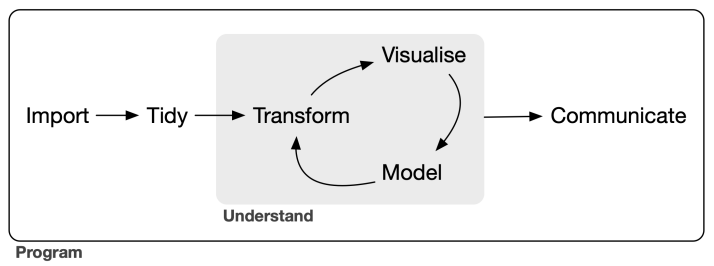
\includegraphics[width = 0.8\textwidth]{graficos/tidyverse_workflow.png}
\caption[Flujo de trabajo en un proyecto de \textit{data science}]{Flujo de trabajo en un proyecto de \textit{data science}. \it Fuente: \citet{tidyversepackage}.}
\label{fig:tidiverse_workflow}
\end{figure}

Para la modelización se ha utilizado \emph{tidymodels}
\citep{tidymodelspackage}. Se trata de un conjunto de paquetes de \(R\)
orientados a facilitar el flujo de trabajo en el modelado estadístico de
datos, siguiendo la filosofía \emph{``tidy data''} de \emph{tidyverse}.
Integra herramientas para ingeniería de características
(\emph{recipes}), definición y ajuste de modelos (\emph{parsnip}),
combinación de flujos de trabajo (\emph{workflows}), partición de datos
y validación cruzada (\emph{rsample}), cálculo de métricas de
rendimiento (\emph{yardstick}), optimización de hiperparámetros
(\emph{tune}) y conversión de resultados de modelos a formatos ordenados
(\emph{broom}). Los paquetes que componen \emph{tidymodels} no
implementan los modelos estadísticos por sí mismos, sino que los
importan de librerías específicas. En su lugar, se enfocan en facilitar
el flujo de trabajo del modelado, mejorando la cohesión y la eficiencia,
a través de una fachada común para la diversidad de paquetes subyacentes
correspondientes a los distintos modelos, y permitiendo la integración
natural con otros paquetes del \emph{tidyverse}.

\begin{figure*}[h]
  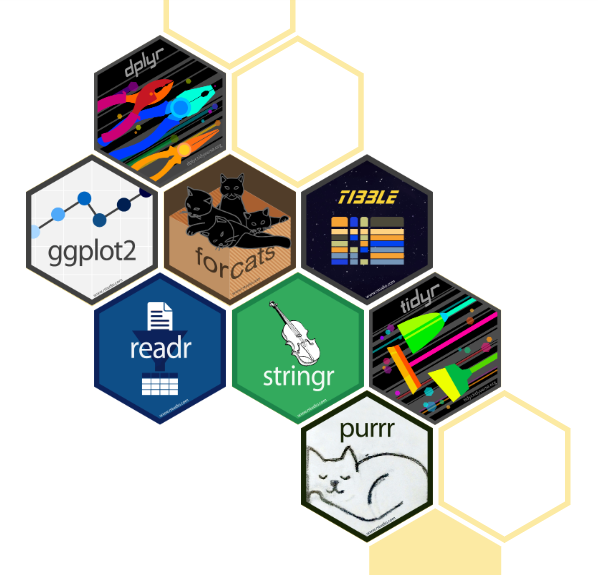
\includegraphics[width=.5\textwidth]{graficos/tidyverse_icons.png}\hfill
  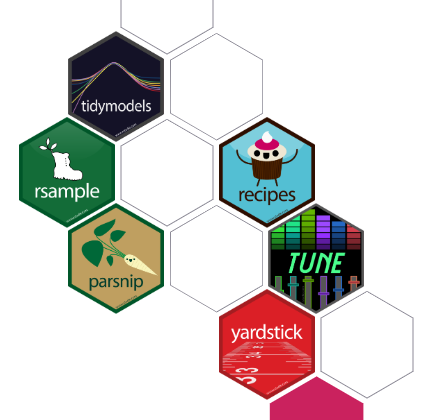
\includegraphics[width=.5\textwidth]{graficos/tidymodels_icons.png}\hfill
  \caption[Iconos de los principales paquetes incluidos en \textit{tidyverse} y en \textit{tidymodels}]{Iconos de los principales paquetes incluidos en \textit{tidyverse} (a la izquierda) y en \textit{tidymodels} (a la derecha). \it Fuente: \url{https://www.tidyverse.org/} para los iconos de tidyverse y \citet{tidymodelspackage} para los iconos de tidymodels.}
\end{figure*}

Como se detalló en la
\protect\hyperlink{datos-georreferenciados}{Sección 2.1 sobre datos
georreferenciados}, para el tratamiento de datos vectoriales se ha
utilizado el paquete de \(R\) \emph{sf} \citep{sfpackage}, que
proporciona una forma estandarizada de codificar y manipular datos
espaciales vectoriales a través de las \emph{simple features},
integrándose dentro del ecosistema \emph{tidyverse}. Para la
manipulación de datos de tipo ráster se ha recurrido al paquete
\emph{terra} \citep{terrapackage}.

La descarga de información meteorológica satelital se ha realizado a
través del paquete \emph{nasapower} \citep{nasapower}, que facilita el
acceso a información meteorológica global de forma reproducible a través
de \(R\). El paquete \emph{mapSpain}\citep{R-mapspain} ha facilitado el
acceso a las fronteras administrativas de España a distintos niveles de
desagregación (comunidad autónoma, provincia y municipio). Se basa en el
\emph{GISCO Eurostat database}
(\url{https://ec.europa.eu/eurostat/web/gisco}) y en el \emph{CartoBase
SIANE} del Instituto Geográfico Nacional (\url{https://www.ign.es/}).

\bibliography{bib/library.bib,bib/paquetes.bib}


%


\end{document}
